\documentclass[12pt]{article}
\usepackage{times} 			% use Times New Roman font

\usepackage[margin=1in]{geometry}   % sets 1 inch margins on all sides
\usepackage{hyperref}               % for URL formatting
\usepackage[pdftex]{graphicx}       % So includegraphics will work
\setlength{\parskip}{1em}           % skip 1em between paragraphs
\usepackage{indentfirst}            % indent the first line of each paragraph
\usepackage{datetime}
\usepackage[small, bf]{caption}
\usepackage{listings}               % for code listings
\usepackage{xcolor}                 % for styling code
\usepackage{multirow}

%New colors defined below
\definecolor{backcolour}{RGB}{246, 246, 246}   % 0xF6, 0xF6, 0xF6
\definecolor{codegreen}{RGB}{16, 124, 2}       % 0x10, 0x7C, 0x02
\definecolor{codepurple}{RGB}{170, 0, 217}     % 0xAA, 0x00, 0xD9
\definecolor{codered}{RGB}{154, 0, 18}         % 0x9A, 0x00, 0x12

%Code listing style named "gcolabstyle" - matches Google Colab
\lstdefinestyle{gcolabstyle}{
  basicstyle=\ttfamily\small,
  backgroundcolor=\color{backcolour},   
  commentstyle=\itshape\color{codegreen},
  keywordstyle=\color{codepurple},
  stringstyle=\color{codered},
  numberstyle=\ttfamily\footnotesize\color{darkgray}, 
  breakatwhitespace=false,         
  breaklines=true,                 
  captionpos=b,                    
  keepspaces=true,                 
  numbers=left,                    
  numbersep=5pt,                  
  showspaces=false,                
  showstringspaces=false,
  showtabs=false,                  
  tabsize=2
}

\lstset{style=gcolabstyle}      %set gcolabstyle code listing

% to make long URIs break nicely
\makeatletter
\g@addto@macro{\UrlBreaks}{\UrlOrds}
\makeatother

% for fancy page headings
\usepackage{fancyhdr}
\setlength{\headheight}{13.6pt} % to remove fancyhdr warning
\pagestyle{fancy}
\fancyhf{}
\rhead{\small \thepage}
\lhead{\small HW\#9, TOMAR}  % EDIT THIS, REPLACE # with HW number
\chead{\small CS 532, Spring 2023} 

%-------------------------------------------------------------------------
\begin{document}

\begin{centering}
{\large\textbf{HW\#9 - Email Classification }}\\ % EDIT THIS
                                % REPLACE # with HW num and ADD title
PRASHANT TOMAR\\                     % EDIT THIS
04/21/2023\\                      % EDIT THIS
\end{centering}

%-------------------------------------------------------------------------

\section*{Q1 - Create two datasets, Testing and Training.}

\subsection*{Answer}
In the root folder of the source code, I have established two main directories: one for training data and the other for testing data. Each of these directories contains two more subdirectories named "on topic" and "off topic", which correspond to our email dataset. To create the on-topic email dataset, I utilized my official email address from Old Dominion University, which includes the university's newsletters and seminar invitations. For the off-topic dataset, I utilized my personal email account, where I receive various advertisements such as new movie releases and release notes . For training, I have produced at least 20 on-topic and 20 off-topic email datasets.

The same process was followed for the testing dataset, but with only 5 on-topic and 5 off-topic datasets. By doing so, we will have a total of 10 training datasets, making it easier to evaluate the results of our classification model.
\\


\begin{figure}[h]
\caption{Folder Structure}
\centering
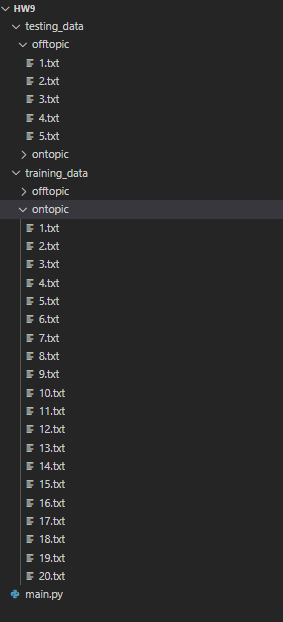
\includegraphics[width=0.25\textwidth]{pic1.png}
\end{figure}
\clearpage

\section*{Q2 - Naive Bayes classifier}

\subsection*{Answer}
The text documents were classified using the code for classification from the book Programming Collective Intelligence. To do this, the files from the training folder were read and a list called list\_train\_data was created. This list contained items with a text property and a class property. The email text was added to the text property, and the class property was set to either "on topic" or "off topic".

After generating a complete list of 40 items, the sample train function from the code was used to train all the items by iterating over the list and sending each item to the training function.

Once the model was trained, the classify function was used to classify the test data by sending it into the function. The function returned the classification based on the trained model classification. Below is the complete implementation.
\\
\begin{lstlisting}[language=Python, caption=Email Classification Using Naive Bayes Classifier] 
import sqlite3 as sqlite
import re
import math
import os


def getwords(doc):
    splitter = re.compile('\W+')
    words = [s.lower() for s in splitter.split(doc)
             if len(s) > 2 and len(s) < 20]
    uniq_words = dict([(w, 1) for w in words])
    return uniq_words


class basic_classifier:

    def __init__(self, getfeatures, filename=None):
        self.fc = {}
        self.cc = {}
        self.getfeatures = getfeatures

    def incf(self, f, cat):
        self.fc.setdefault(f, {})
        self.fc[f].setdefault(cat, 0)
        self.fc[f][cat] += 1

    def incc(self, cat):
        self.cc.setdefault(cat, 0)
        self.cc[cat] += 1

    def fcount(self, f, cat):
        if f in self.fc and cat in self.fc[f]:
            return float(self.fc[f][cat])
        return 0.0

    def catcount(self, cat):
        if cat in self.cc:
            return float(self.cc[cat])
        return 0

    def totalcount(self):
        return sum(self.cc.values())

    def categories(self):
        return self.cc.keys()

    def train(self, item, cat):
        features = self.getfeatures(item)
        for f in features:
            self.incf(f, cat)
        self.incc(cat)

    def fprob(self, f, cat):
        if self.catcount(cat) == 0:
            return 0
        return self.fcount(f, cat)/self.catcount(cat)

    def weightedprob(self, f, cat, prf, weight=1.0, ap=0.5):
        basicprob = prf(f, cat)
        totals = sum([self.fcount(f, c) for c in self.categories()])
        bp = ((weight*ap)+(totals*basicprob))/(weight+totals)
        return bp


class naivebayes(basic_classifier):

    def __init__(self, getfeatures):
        basic_classifier.__init__(self, getfeatures)
        self.thresholds = {}

    def docprob(self, item, cat):
        features = self.getfeatures(item)
        p = 1
        for f in features:
            p *= self.weightedprob(f, cat, self.fprob)
        return p

    def prob(self, item, cat):
        catprob = self.catcount(cat)/self.totalcount()
        docprob = self.docprob(item, cat)
        return docprob*catprob

    def setthreshold(self, cat, t):
        self.thresholds[cat] = t

    def getthreshold(self, cat):
        if cat not in self.thresholds:
            return 1.0
        return self.thresholds[cat]

    def classify(self, item, default=None):
        probs = {}
        max = 0.0
        for cat in self.categories():
            probs[cat] = self.prob(item, cat)
            if probs[cat] > max:
                max = probs[cat]
                best = cat
        for cat in probs:
            if cat == best:
                continue
            if probs[cat]*self.getthreshold(best) > probs[best]:
                return default
        return best


all_training_ontopic_files = os.listdir('training_data\ontopic')
all_training_offtopic_files = os.listdir('training_data\offtopic')
all_testing_ontopic_files = os.listdir('testing_data\ontopic')
all_testing_offtopic_files = os.listdir('testing_data\offtopic')

list_train_data = []

for item in all_training_ontopic_files:
    fd = open('training_data\ontopic\\' + item, 'r', encoding="utf8")
    text = fd.read()
    train_data = {'text': text, 'class': 'on topic'}
    list_train_data.append(train_data)

for item in all_training_offtopic_files:
    fd = open('training_data\offtopic\\' + item, 'r', encoding="utf8")
    text = fd.read()
    train_data = {'text': text, 'class': 'off topic'}
    list_train_data.append(train_data)


def sampletrain(cl):
    for item in list_train_data:
        cl.train(item['text'], item['class'])
    

cl = naivebayes(getwords)
sampletrain(cl)

list_testing_ontopic_data = []
for item in all_testing_ontopic_files:
    fd = open('testing_data\ontopic\\' + item, 'r', encoding="utf8")
    text = fd.read()
    train_data = {'text': text, 'class': 'on topic'}
    list_testing_ontopic_data.append(train_data)

list_testing_offtopic_data = []
for item in all_testing_offtopic_files:
    fd = open('testing_data\offtopic\\' + item, 'r', encoding="utf8")
    text = fd.read()    
    train_data = {'text': text, 'class': 'off topic'}
    list_testing_offtopic_data.append(train_data)

print(cl.classify(list_testing_ontopic_data[0]['text'], default='unknown'))
print(cl.classify(list_testing_ontopic_data[1]['text'], default='unknown'))
print(cl.classify(list_testing_ontopic_data[2]['text'], default='unknown'))
print(cl.classify(list_testing_ontopic_data[3]['text'], default='unknown'))
print(cl.classify(list_testing_ontopic_data[4]['text'], default='unknown'))

print(cl.classify(list_testing_offtopic_data[0]['text'], default='unknown'))
print(cl.classify(list_testing_offtopic_data[1]['text'], default='unknown'))
print(cl.classify(list_testing_offtopic_data[2]['text'], default='unknown'))
print(cl.classify(list_testing_offtopic_data[3]['text'], default='unknown'))
print(cl.classify(list_testing_offtopic_data[4]['text'], default='unknown'))


\end{lstlisting}
\\
After running the code, the output was displayed in the terminal window. The results were accurate, and the classifier was able to correctly classify all the data. You can find the results in the table on the next page.

\begin{table}[h]
\centering
\caption{Classification of the Email}
\label{tbl:simple}
\begin{tabular}{p{0.10\linewidth}p{0.20\linewidth}p{0.20\linewidth}p{0.10\linewidth}}
\hline
\textbf{Email} & \textbf{Actual Result} & \textbf{Predicted Result}\\ \hline \hline
1   &      On Topic  &       On Topic   \\ \hline
2   &      On Topic  &       On Topic   \\ \hline 
3   &      On Topic  &       On Topic   \\ \hline
4   &      On Topic  &       On Topic   \\ \hline
5   &      On Topic  &       On Topic   \\ \hline
6   &      Off Topic  &       Off Topic   \\ \hline
7   &      Off Topic  &       Off Topic   \\ \hline
8   &      Off Topic  &       Off Topic   \\ \hline
9   &      Off Topic  &       Off Topic   \\ \hline
10   &     Off Topic  &       Off Topic   \\ \hline \hline
\end{tabular}
\end{table}

\\
\clearpage

\section*{Q3 - Confusion Matrix}

\subsection*{Answer}

As evident from the Q2 results, I have obtained a 100\% accuracy rate. Please refer to the confusion matrix presented below.

\begin{table}[h]
\centering
\caption{Example Confusion Matrix from Wikipedia}
\label{tbl:confusion}
\begin{tabular}{l|l|c|c|}
\multicolumn{2}{c}{}&\multicolumn{2}{c}{Actual}\\
\cline{3-4}
\multicolumn{2}{c|}{}&On Topic&Off Topic\\
\cline{2-4}
\multirow{2}{*}{Predicted}& On Topic & 5 (TP) & 0 (FP)\\
\cline{2-4}
& Off Topic & 0 (FN) & 5 (TN) \\
\cline{2-4}
\end{tabular}
\end{table}
\\
\\
Upon examining the confusion matrix, it is apparent that the Bayes classifier performed exceptionally well and achieved 100\% accuracy. However, it was expected that there would be some variation in the results as I had included off-topic data from my personal email address in the training dataset as mentioned in Q1. Specifically, I had received a newsletter from a different university during the time I was applying to Old Dominion University, and I was hoping that this off-topic email would be classified as on-topic.

 
\clearpage
\section*{References}



\begin{itemize}
    \item {Code Ref from Chap 6, \url{https://learning.oreilly.com/library/view/programming-collective-intelligence/9780596529321/}}
\end{itemize}

\end{document}

